
\section{Catalan characterization}
\label{sec:catalan:characterization}

In this section we tackle a modular characterization, using congruence relation
$\equiv_{2}$, for the Catalan array $\mathcal{C}$ from a formal point of view.
We aim at a proof driven by
\autoref{fig:catalan-traditional-standard-ignore-negatives-centered-colouring-127-rows-mod2-partitioning-triangle},
and, in order to fullfil it, we proceed \emph{piece-wise} breaking such
characterization into the following sections, where an independent region of
$\mathcal{C}_{\equiv_{2}}$ is described in each one of them.


\subsection{On the very first column of $\mathcal{C}_{\equiv_{2}}$}

In this section we want to characterize the very first column $\vect{c}_{0}$
of $\mathcal{C}_{\equiv_{2}}$, namely the column composed of Catalan numbers only,
formally $C_{j}=c_{j,0}\in\vect{c}_{0}$, for any $j\in\mathbb{N}$:
for the sake of clarity, in \autoref{fig:catalan-first-column} segment
$\diagup_{\lbrace 0,1,2,\ldots,2^{4}\rbrace}^{0}$ of $\vect{c}_{0}\subset\mathcal{C}_{\equiv_{2}}$
is highlighted. In the proof, congruence relation $\equiv_{2}$ is applied to \autoref{eq:catalan:coeff:rewriting};
moreover, we write $j$ in base $2$, so there exists $k\in\mathbb{N}$ such that
$j=j_{0} + j_{1}\,2 + j_{2}\,2^{2} + \ldots + j_{k}\,2^{k}$, where
$j_{r}\in\lbrace0,1\rbrace$, for each $r\in\lbrace0,\ldots,k\rbrace$.

\begin{theorem}
    Let $j\in\mathbb{N}$, then $C_{j} \equiv_{2} 0$ unless $j=2^{\alpha}-1$ for some $\alpha\in\mathbb{N}$,
    in which case $C_{2^{\alpha}-1} \equiv_{2} 1$ holds.
\end{theorem}

\begin{proof}
We start with the boundary case for $j=0$, then $C_{0} \equiv_{2} 1$ because for the subscript $j=0$
there is $\alpha=0$ so that $j = 2^{\alpha}-1$. On the contrary, for $j>0$ %in order to apply Lucas theorem,
we proceed by cases on $j$'s parity:
\begin{itemize}
    \item let $j=2\alpha$, for some $\alpha\in\mathbb{N}$, so $j_{0}=0$,
        which make vanish the subtrahend of \autoref{eq:catalan:coeff:rewriting}:
        \begin{displaymath}
            {{2j}\choose{j+1}}
            \equiv_{2} {{0}\choose{1}}{{0}\choose{j_{1}}}{{j_{1}}\choose{j_{2}}}
                \ldots{{j_{k-1}}\choose{j_{k}}}{{j_{k}}\choose{0}}\equiv_{2}0
        \end{displaymath}
        Also the minuend vanishes:
        \begin{displaymath}
            C_{j}\equiv_{2}{{2j}\choose{j}}
            \equiv_{2} {{0}\choose{0}}{{0}\choose{j_{1}}}{{j_{1}}\choose{j_{2}}}
                \ldots{{j_{k-1}}\choose{j_{k}}}{{j_{k}}\choose{0}}\equiv_{2}0
        \end{displaymath}
        A boundary case pops out when $\alpha=0$ where $j$ has to be written as
        $j=0 + 0\cdot2 + 0\cdot2^{2} + \ldots + 0\cdot2^{k}$, therefore:
        \begin{displaymath}
            C_{0}\equiv_{2}{{0}\choose{0}}
            \equiv_{2} {{0}\choose{0}}{{0}\choose{0}}{{0}\choose{0}}
                \ldots{{0}\choose{0}}{{0}\choose{0}}\equiv_{2}1
        \end{displaymath}
        this is indeed the only case where $C_{2\alpha} \equiv_{2}1$.
        \iffalse
        \begin{proof}
            Assume not, hence there exists $\hat{\alpha}\in\mathbb{N}$, greater than $0$,
            such that $C_{2\hat{\alpha}} \equiv_{2}1$. So for ${{0}\choose{j_{1}}}$
            be not zero then $j_{1}=0$; in turn, this constraint requires a new one, namely
            for ${{0}\choose{j_{2}}}$ be not zero then $j_{2}=0$;
            in turn, this constraint requires a new one, namely
            for ${{0}\choose{j_{3}}}$ be not zero then $j_{3}=0$;
            in turn, this constraint requires a new one, namely\ldots
            for ${{0}\choose{j_{k}}}$ be not zero then $j_{k}=0$.
            Therefore $j=0$, which contradicts the hypothesis $\alpha>0$. So,
            for even $j > 0$, coefficient $C_{j}\equiv_{2}0$, as required.
        \end{proof}
        \fi

    \item let $j=2\alpha+1$, for some $\alpha\in\mathbb{N}$, so $j_{0}=1$,
        which make vanish the minuend of \autoref{eq:catalan:coeff:rewriting}:
        \begin{displaymath}
            {{2j}\choose{j}}
            \equiv_{2} {{0}\choose{1}}{{1}\choose{j_{1}}}{{j_{1}}\choose{j_{2}}}
                \ldots{{j_{k-1}}\choose{j_{k}}}{{j_{k}}\choose{0}}\equiv_{2}0
        \end{displaymath}
        so:
        \begin{displaymath}
            C_{j}\equiv_{2}-{{2j}\choose{j+1}}.
            %\equiv_{2} {{0}\choose{0}}{{0}\choose{j_{1}}}{{j_{1}}\choose{j_{2}}}
                %\ldots{{j_{k-1}}\choose{j_{k}}}{{j_{k}}\choose{0}}\equiv_{2}0
        \end{displaymath}
        Now observe that $(-1)^{-1}\mod2$, the multiplicative inverse of $-1$, equals $1$
        since $(-1)\cdot 1 \equiv_{2}1$, therefore we can multiply both members by
        $(-1)^{-1}\mod2$ to get:
        \begin{displaymath}
            C_{j}\equiv_{2}{{2j}\choose{j+1}}.
            %\equiv_{2} {{0}\choose{0}}{{0}\choose{j_{1}}}{{j_{1}}\choose{j_{2}}}
                %\ldots{{j_{k-1}}\choose{j_{k}}}{{j_{k}}\choose{0}}\equiv_{2}0
        \end{displaymath}

        Careful handling is necessary for the term $j+1$:
        since $j$ is odd by hypothesis, increasing it could yield a chain of carries.
        So, handling $j+1$ in a generic way, we write
        $j$ in base $2$ in its most general form, putting evidence on coefficients:
        \begin{displaymath}
            j=\left(\underbrace{1,1,\ldots,1}_{\beta},0,j_{\beta+1},\ldots,j_{\beta+\gamma}\right)_{2}
        \end{displaymath}
        where $\beta,\gamma\in\mathbb{N}$ such that $\beta>0$ and $\beta+\gamma=k$.
        Incrementing $j$ by $1$ we get
        \begin{displaymath}
            j+1=\left(\underbrace{0,0,\ldots,0}_{\beta},1,j_{\beta+1},\ldots,j_{\beta+\gamma}%,j_{\beta+\gamma+1}
                \right)_{2}
        \end{displaymath}
        so the congruence relation gets the shape
        \begin{displaymath}
            %\hspace{-2cm}
            C_{j}\equiv_{2}{{2j}\choose{j+1}}
                \equiv_{2} \underbrace{{{0}\choose{0}}{{1}\choose{0}}
                {{1}\choose{0}}\ldots{{1}\choose{0}}}_{\beta}
                    {{1}\choose{1}}{{0}\choose{j_{\beta+1}}}{{j_{\beta+1}}\choose{j_{\beta+2}}}
                    \ldots{{j_{\beta+\gamma-1}}\choose{j_{\beta+\gamma}}}{{j_{\beta+\gamma}}\choose{0}}%{\beta+\gamma+1}}
        \end{displaymath}
        and a simplification yield
        \begin{displaymath}
            C_{j}\equiv_{2} {{0}\choose{j_{\beta+1}}}
                {{j_{\beta+1}}\choose{j_{\beta+2}}}
                    \ldots{{j_{\beta+\gamma-1}}\choose{j_{\beta+\gamma}}}.
        \end{displaymath}
        At last, $C_{j}\equiv_{2} 1$ holds if coefficients
            $j_{\beta+1}, \ldots, j_{\beta+\gamma-1},j_{\beta+\gamma}$
        are $0$ them all, which implies that
        \begin{displaymath}
            j=\left(\underbrace{1,1,\ldots,1}_{\beta},\underbrace{0,0,\ldots,0}_{k-\beta+1}\right)_{2},
        \end{displaymath}
        in other words $j = 2^{\beta+1}-1$. As boundary case, to handle $C_{1}$ correctly
        (the above result doesn't cover it because $\beta>0$) observe that
        \begin{displaymath}
            C_{1}\equiv_{2} {{2}\choose{2}}\equiv_{2} {{0}\choose{0}}{{1}\choose{1}}\equiv_{2}1,
        \end{displaymath}
        as required.
\end{itemize}
\end{proof}

It is interesting to observe that if we use the ``traditional'' closed formula
for a Catalan coefficient $C_{j}$:
\begin{displaymath}
    (j+1)\,C_{j} = {{2j}\choose{j}}
\end{displaymath}
where $j=2\alpha+1$, it would have been hard to handle, because:
\begin{displaymath}
    2(\alpha+1)\,C_{j}\equiv_{2} {{0}\choose{1}}{{1}\choose{j_{1}}}
            \ldots{{j_{k-1}}\choose{j_{k}}} \equiv_{2} 0
\end{displaymath}
reduces to $0\equiv_{2}0$, giving no opportunity to derive any
property about coefficient $C_{j}$.


\begin{figure}[p]

    \noindent\makebox[\textwidth]{
        \centering
        %\includegraphics[width=0.8\textwidth]{../../sympy/catalan/coloured.pdf}

        % using *angle* property to rotate it is difficult to properly align it
        % in order to have a "real" matrix representation.
        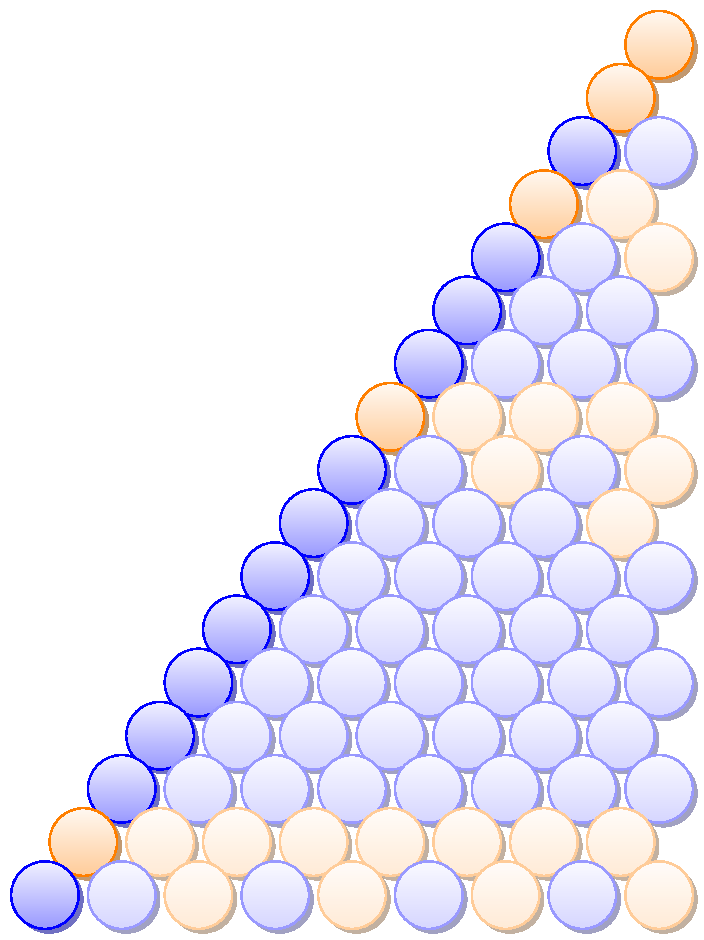
\includegraphics[
            width=7cm, 
            height=6cm, 
            keepaspectratio=true]{catalan-tikz/first-column/first-column.pdf}
    }

    % this 'particular' line is necessary to use `displaymath' environment
    % into the caption environment, togheter with the inclusion of 
    % `caption' package. See here for more explanation:
    % http://stackoverflow.com/questions/2716227/adding-an-equation-or-formula-to-a-figure-caption-in-latex
    \captionsetup{singlelinecheck=off}
    \caption[.]{ \textcolor{blue}{even},
        \textcolor{orange}{odd}  }

    \label{fig:catalan-first-column}

\end{figure}


\subsection{On rows composed of \emph{odd} coefficients only}

\begin{theorem}
    Every row $\vect{r}_{2^{\alpha}-1}$ of $\mathcal{C}_{\equiv_{2}}$, with index $2^{\alpha}-1$,
    is composed of \emph{odd} coefficients only, for $\alpha\in\mathbb{N}$.
    \label{thm:odd:coeff:only:on:last:but:one:row}
\end{theorem}

\begin{proof}
    Choose any $\alpha\in\mathbb{N}$. The very first coefficient $d_{2^{\alpha}-1,0}$
    lying on row $\vect{r}_{2^{\alpha}-1}$ satisfies $d_{2^{\alpha}-1,0}\equiv_{2}1$. 
    What about $d_{2^{\alpha}-1,1}$?  Recall that we can write it according to
    \autoref{eq:convolution:expansion:for:generic:element:in:catalan:array} as
    \begin{displaymath}
        d_{2^{\alpha}-1,1} = \sum_{i_{1}+ i_{2}=2^{\alpha}}{ C_{i_{1}-1}\,C_{i_{2}-1} }
    \end{displaymath}
    hence %indices $i_{1}$ and $i_{2}$ in the summation  
    $2^{\alpha}$ divides $i_{1}+i_{2}$ \emph{exactly}, so
    $\displaystyle 1 = \frac{i_{1}}{2^{\alpha}}+\frac{i_{2}}{2^{\alpha}}$ for 
            $i_{1},i_{2}\in\lbrace 0,\ldots,2^{\alpha}\rbrace$;
    %, which is the same to say that
    %$\frac{i_{1}}{2^{\alpha}}$ and $\frac{i_{2}}{2^{\alpha}}$ are both integers.
    this implies that there exists $\beta,\gamma\in\mathbb{N}$ both lesser or
    equal to  $\alpha$, such that $i_{1}=2^{\beta}$ and $i_{2}=2^{\gamma}$,
    respectively; by this fact, it follows that $C_{i_{1}-1}=C_{2^{\beta}-1}\equiv_{2}1$ and
    $C_{i_{2}-1}=C_{2^{\gamma}-1}\equiv_{2}1$, therefore $C_{i_{1}-1}\,C_{i_{2}-1}\equiv_{2}1$.

    By construction, if one index in
    $i_{1}+ i_{2}=2^{\alpha}$ gets fixed then the other does the same as well;
    in particular, there are $2^{\alpha}+1$ available choices for the first index and only 
    $1$ for the second, formally
    \begin{displaymath}
        d_{2^{\alpha}-1,1} = \sum_{i_{1}+ i_{2}=2^{\alpha}}{ C_{i_{1}-1}\,C_{i_{2}-1} }
            \equiv_{2} \sum_{k=1}^{2^{\alpha}+1}{1}\equiv_{2} 2^{\alpha}+1\equiv_{2} 1\,.
    \end{displaymath}

    On the other hand, we write an arbitrary coefficient $d_{2^{\alpha}-1,s}$, where
    $s\in\lbrace{2,\ldots,2^{\alpha}-1}\rbrace$, as
    \begin{displaymath}
        d_{2^{\alpha}-1,s} = \sum_{i_{1}+i_{2}+\ldots+i_{s+1}=2^{\alpha}}
            {C_{i_{1}-1}\,C_{i_{2}-1}\ldots\,C_{i_{s+1}-1}}
    \end{displaymath}
    in order to repeat an argument similar to the previous one. In
    $\displaystyle 1 = \frac{i_{1}}{2^{\alpha}}+\ldots+\frac{i_{s+1}}{2^{\alpha}}$ there exists one
    index $i_{j}\in\lbrace 0,\ldots,2^{\alpha}\rbrace$ such that satisfies
    $i_{j}=2^{\alpha_{j}}$, for some $\alpha_{j}\leq\alpha$, which entails
    $C_{i_{j}-1}\equiv_{2}1$, for $j\in\lbrace1,\ldots,s+1\rbrace$. Therefore the congruences
    \begin{displaymath}
        d_{2^{\alpha}-1,s} \equiv_{2} \sum_{i_{1}+i_{2}+\ldots+i_{s+1}=2^{\alpha}}{1}
            \equiv_{2} {{s+2^{\alpha}}\choose{2^{\alpha}}},
    \end{displaymath}
    hold because the summation over indices $i_{1},\ldots,i_{s+1}$ asks to count the
    number of $2^{\alpha}$-combinations of $s+1$ distinct objects each of
    which may appear indefinitely often, in particular from $0$ to $2^{\alpha}$ times,
    hence the sought number is ${{(s+1)+2^{\alpha}-1}\choose{2^{\alpha}}}$
    according to \cite[equation 10 at page 7]{riordan:intro:combinatorial:analysis}.

    Again, we are interested in the parity of such coefficient, therefore
    write $s=s_{0}+s_{1}\,2+\ldots+s_{\alpha-1}\,2^{\alpha-1}$, because $s$ can equal
    $2^{\alpha}-1$ at most, and the application of the Lucas theorem yields
    \begin{displaymath}
        {{s+2^{\alpha}}\choose{2^{\alpha}}}\equiv_{2}
            {{s_{0}}\choose{0}}{{s_{1}}\choose{0}} \ldots
                {{s_{\alpha-1}}\choose{0}}{{1}\choose{1}}\equiv_{2}1
    \end{displaymath}
    which, in turn, entails that each coefficient lying on a row
    $\vect{r}_{2^{\alpha}-1}$ is odd, as required.
\end{proof}


\begin{figure}[p]

    \noindent\makebox[\textwidth]{
        \centering
        %\includegraphics[width=0.8\textwidth]{../../sympy/catalan/coloured.pdf}

        % using *angle* property to rotate it is difficult to properly align it
        % in order to have a "real" matrix representation.
        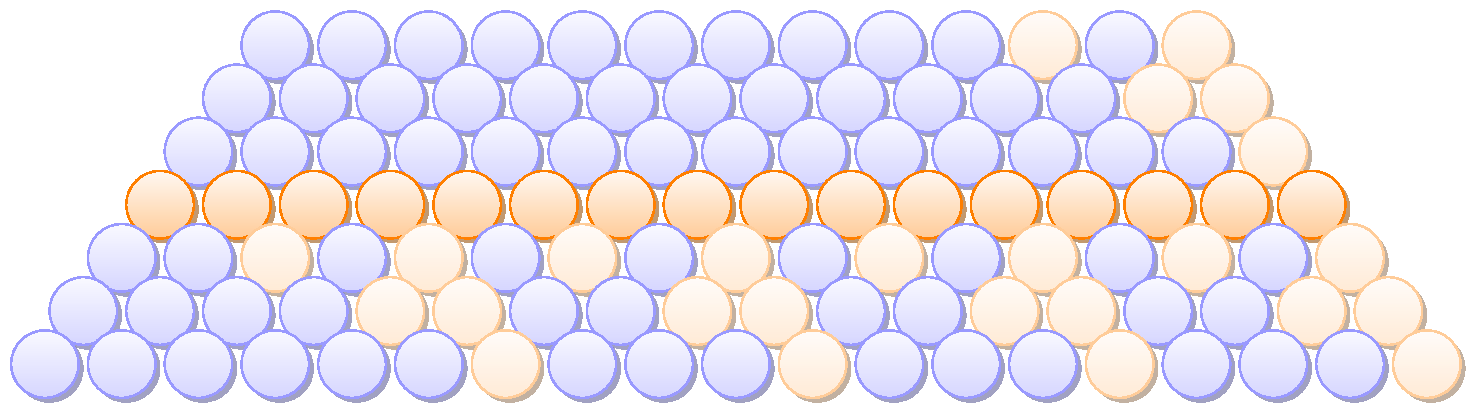
\includegraphics[width=10cm, height=10cm, keepaspectratio=true]
            {../RART2015/catalan-tikz/odd-row/odd-row.pdf}
    }

    % this 'particular' line is necessary to use `displaymath' environment
    % into the caption environment, togheter with the inclusion of 
    % `caption' package. See here for more explanation:
    % http://stackoverflow.com/questions/2716227/adding-an-equation-or-formula-to-a-figure-caption-in-latex
    \captionsetup{singlelinecheck=off}
    \caption[Row $\vect{r}_{2^{4}-1}$ of $\mathcal{C}_{\equiv_{2}}$]{
        Row $\vect{r}_{2^{4}-1}$ composed of coefficients $\textcolor{orange}{d_{2^{4}-1,s} \equiv_{2} 1}$, 
        for $s\in\lbrace1,\ldots,2^{4}-1 \rbrace$ }

    \label{fig:catalan-odd-row}

\end{figure}

In \autoref{fig:catalan-odd-row} row $\vect{r}_{2^{4}-1}$ is highlighted.

\subsection{On rows composed of odd and even coefficients}

\begin{theorem}
    Let $\vect{r}_{2^{\alpha}}$ be a row of $\mathcal{C}_{\equiv_{2}}$,
    for some $\alpha\in\mathbb{N}$. Then, excluded the very first coefficient
    $d_{2^{\alpha},0}$ which is even, $\vect{r}_{2^{\alpha}}$ is composed of
    alternating even and odd coefficients. Formally:
    \begin{displaymath}
        d_{2^{\alpha},j}\equiv_{2}0 \leftrightarrow j = 2k+1
    \end{displaymath}
    for some $k\in\mathbb{N}$.
\end{theorem}

\begin{proof}
    Let $d_{2^{\alpha},j}$ be a coefficient lying on row $\vect{r}_{2^{\alpha}}$,
    for some $j\in\lbrace1,\ldots,2^{\alpha}\rbrace$. Since $\mathcal{C}$'s $A$-sequence is:
    \begin{displaymath}
        A_{\mathcal{C}}(t)=\frac{1}{1-t}=1+t+t^{2}+t^{3}+t^{4}+t^{5}+t^{6}+t^{7}+t^{8}+
            \mathcal{O}(t^{9})
    \end{displaymath}
    it follows that $d_{2^{\alpha},j}$ can be written as the combination of $r+2$
    coefficients lying on the previous row, namely $\vect{r}_{2^{\alpha}-1}$:
    \begin{displaymath}
        d_{2^{\alpha},j} = d_{2^{\alpha}-1,j-1} +d_{2^{\alpha}-1,j} +\ldots+d_{2^{\alpha}-1,j+r}
    \end{displaymath}
    where $r$ satisfies $r=2^{\alpha}-1-j$, so $2^{\alpha}-j+1$ coefficients are
    combined.  By \autoref{thm:odd:coeff:only:on:last:but:one:row},
    row $\vect{r}_{2^{\alpha}-1}$ is composed by \emph{odd}
    coefficients only, therefore proceed by cases on the parity of $j$:
    \begin{itemize}
        \item if $j$ is \emph{odd}, assume $j=2k+1$ for some $k\in\mathbb{N}$, then
            $2^{\alpha}-2k$ coefficients are combined, which is an \emph{even} number.
            Adding an \emph{even} number of \emph{odd} numbers yield an \emph{even} number;
        \item if $j$ is \emph{even}, assume $j=2k$ for some $k\in\mathbb{N}$, then
            $2^{\alpha}-2k+1$ coefficients are combined, which is an \emph{odd} number.
            Adding an \emph{odd} number of \emph{odd} numbers yield an \emph{odd} number.
    \end{itemize}
\end{proof}


\begin{figure}[p]

    \noindent\makebox[\textwidth]{
        \centering
        %\includegraphics[width=0.8\textwidth]{../../sympy/catalan/coloured.pdf}

        % using *angle* property to rotate it is difficult to properly align it
        % in order to have a "real" matrix representation.
        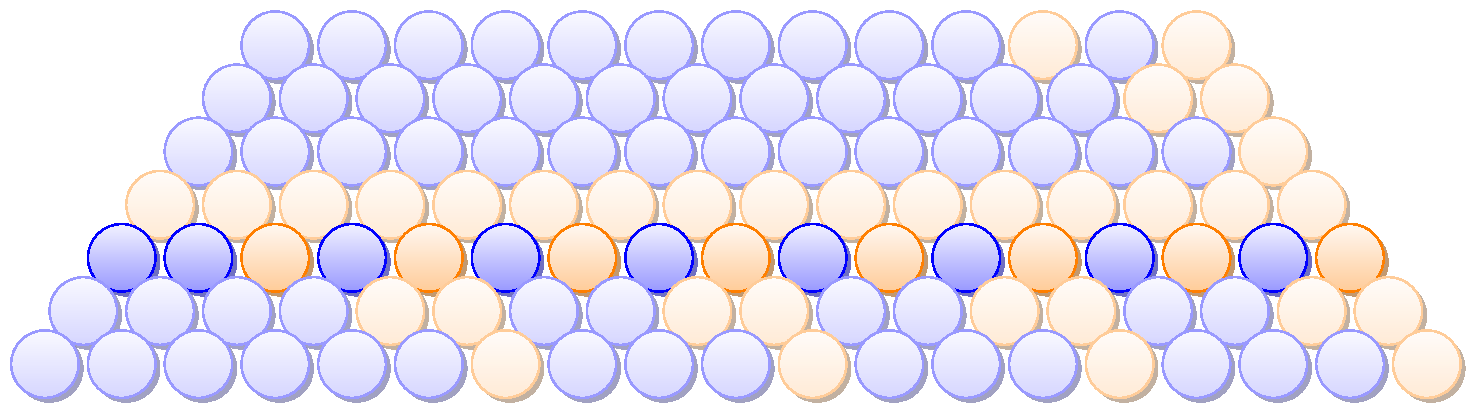
\includegraphics[width=10cm, height=3cm, keepaspectratio=true]{catalan-tikz/odd-row/alternating-row.pdf}
    }

    % this 'particular' line is necessary to use `displaymath' environment
    % into the caption environment, togheter with the inclusion of 
    % `caption' package. See here for more explanation:
    % http://stackoverflow.com/questions/2716227/adding-an-equation-or-formula-to-a-figure-caption-in-latex
    \captionsetup{singlelinecheck=off}
    \caption[.]{Row of coefficients $\textcolor{orange}{d_{2^{4}-1,s}} \equiv_{2} 1$ 
        for $s\in\lbrace1,\ldots,2^{4}-1 \rbrace$ }

    \label{fig:catalan-odd-row}

\end{figure}

In \autoref{fig:catalan-alternating-row} row $\vect{r}_{2^{4}}$ is highlighted.

\subsection{On the \emph{mirror} segment}

Before showing new theorems, we introduce the object
$\Phi^{(\alpha)}$ which denotes a particular segment contained
in the principal cluster $\mathcal{C}^{(\alpha+1)}$.
We call $\Phi^{(\alpha)}$ the \emph{mirror} segment in
$\mathcal{C}^{(\alpha+1)}$ and it is defined as follows:
\begin{displaymath}
    \Phi^{(\alpha)}=\diagup_{\lbrace 1,2,\ldots,2^{\alpha}-1\rbrace}^{2^{\alpha}-1}
\end{displaymath}

\begin{theorem}
    Choose any $\alpha\in\mathbb{N}$, then $\Phi^{(\alpha)}$ satisfies:
    \begin{displaymath}
        d_{s,2^{\alpha}-1}\in\Phi^{(\alpha)} \rightarrow d_{s,2^{\alpha}-1}\equiv_{2}0
    \end{displaymath}
    where $s\in rows\left(\Phi^{(\alpha)}\right)=\lbrace2^{\alpha},\ldots,2^{\alpha+1}-2\rbrace$.
    \label{thm:mirror:segment:definition}
\end{theorem}

\begin{proof}
Let $d_{s,2^{\alpha}-1}$ a coefficient in the segment $\Phi^{(\alpha)}$,
according to \autoref{eq:convolution:expansion:for:generic:element:in:catalan:array}
write it as:
\begin{displaymath}
    d_{s, 2^{\alpha}-1} = \sum_{i_{1}+i_{2}+\ldots+i_{2^{\alpha}}=s+1}
        {C_{i_{1}-1}\,C_{i_{2}-1}\cdots\,C_{i_{2^{\alpha}}-1}}
\end{displaymath}
Observe that, for $s\in\Phi^{(\alpha)}$, the number of Catalan
coefficients multiplied together in each summand is the same, namely
$2^{\alpha}$.  What changes respect to $s$ is the set of values each
index $i_{j}$ can take. In the following table we report instantiated sets
of values, depending on $s$, for both indexes and coefficients:
\begin{displaymath}
    \begin{array}{c|c|c}
        s = 2^{\alpha}
            & i_{j}\in\lbrace0,\ldots,2^{\alpha}+1\rbrace
            & C_{k}\in\lbrace C_{-1},\ldots,C_{2^{\alpha}}\rbrace\\
        s = 2^{\alpha} +1
            & i_{j}\in\lbrace0,\ldots,2^{\alpha}+2\rbrace
            & C_{k}\in\lbrace C_{-1},\ldots,C_{2^{\alpha}+1}\rbrace\\
        \vdots & \vdots&\vdots \\
        s = 2^{\alpha+1} -2
            & i_{j}\in\lbrace0,\ldots,2^{\alpha+1}-1\rbrace
            & C_{k}\in\lbrace C_{-1},\ldots,C_{2^{\alpha+1}-2}\rbrace\\
    \end{array}
\end{displaymath}
Set $\lbrace C_{-1},\ldots,C_{2^{\alpha}}\rbrace$ and set
$\lbrace C_{-1},\ldots,C_{2^{\alpha+1}-2}\rbrace$ are the smaller and the bigger one, respectively, and
have the same subset $\Omega^{(\alpha)}$ of \emph{odd} coefficients:
\begin{displaymath}
    \Omega^{(\alpha)}=\lbrace C_{-1}, C_{2^{\alpha-(\alpha-1)}-1},C_{2^{\alpha-(\alpha-2)}-1},\ldots,
        C_{2^{\alpha-1}-1},C_{2^{\alpha}-1}\rbrace
\end{displaymath}
where $\left|\Omega^{(\alpha)}\right|=\alpha+1$.
Since each summand term $C_{i_{1}-1}\,C_{i_{2}-1}\ldots\,C_{i_{2^{\alpha}}-1}$
has $2^{\alpha}$ coefficients, no matter if it contains each coefficient in $\Omega^{(\alpha)}$ and,
more importantly, one of them cannot belong to $\Omega^{(\alpha)}$:
the remaining ones make it vanish and $d_{s, 2^{\alpha}-1} \equiv_{2} 0$, for any suitable $s$,
as required.

\end{proof}


\begin{figure}[htb]

    \noindent\makebox[\textwidth]{
        \centering
        %\includegraphics[width=0.8\textwidth]{../../sympy/catalan/coloured.pdf}

        % using *angle* property to rotate it is difficult to properly align it
        % in order to have a "real" matrix representation.
        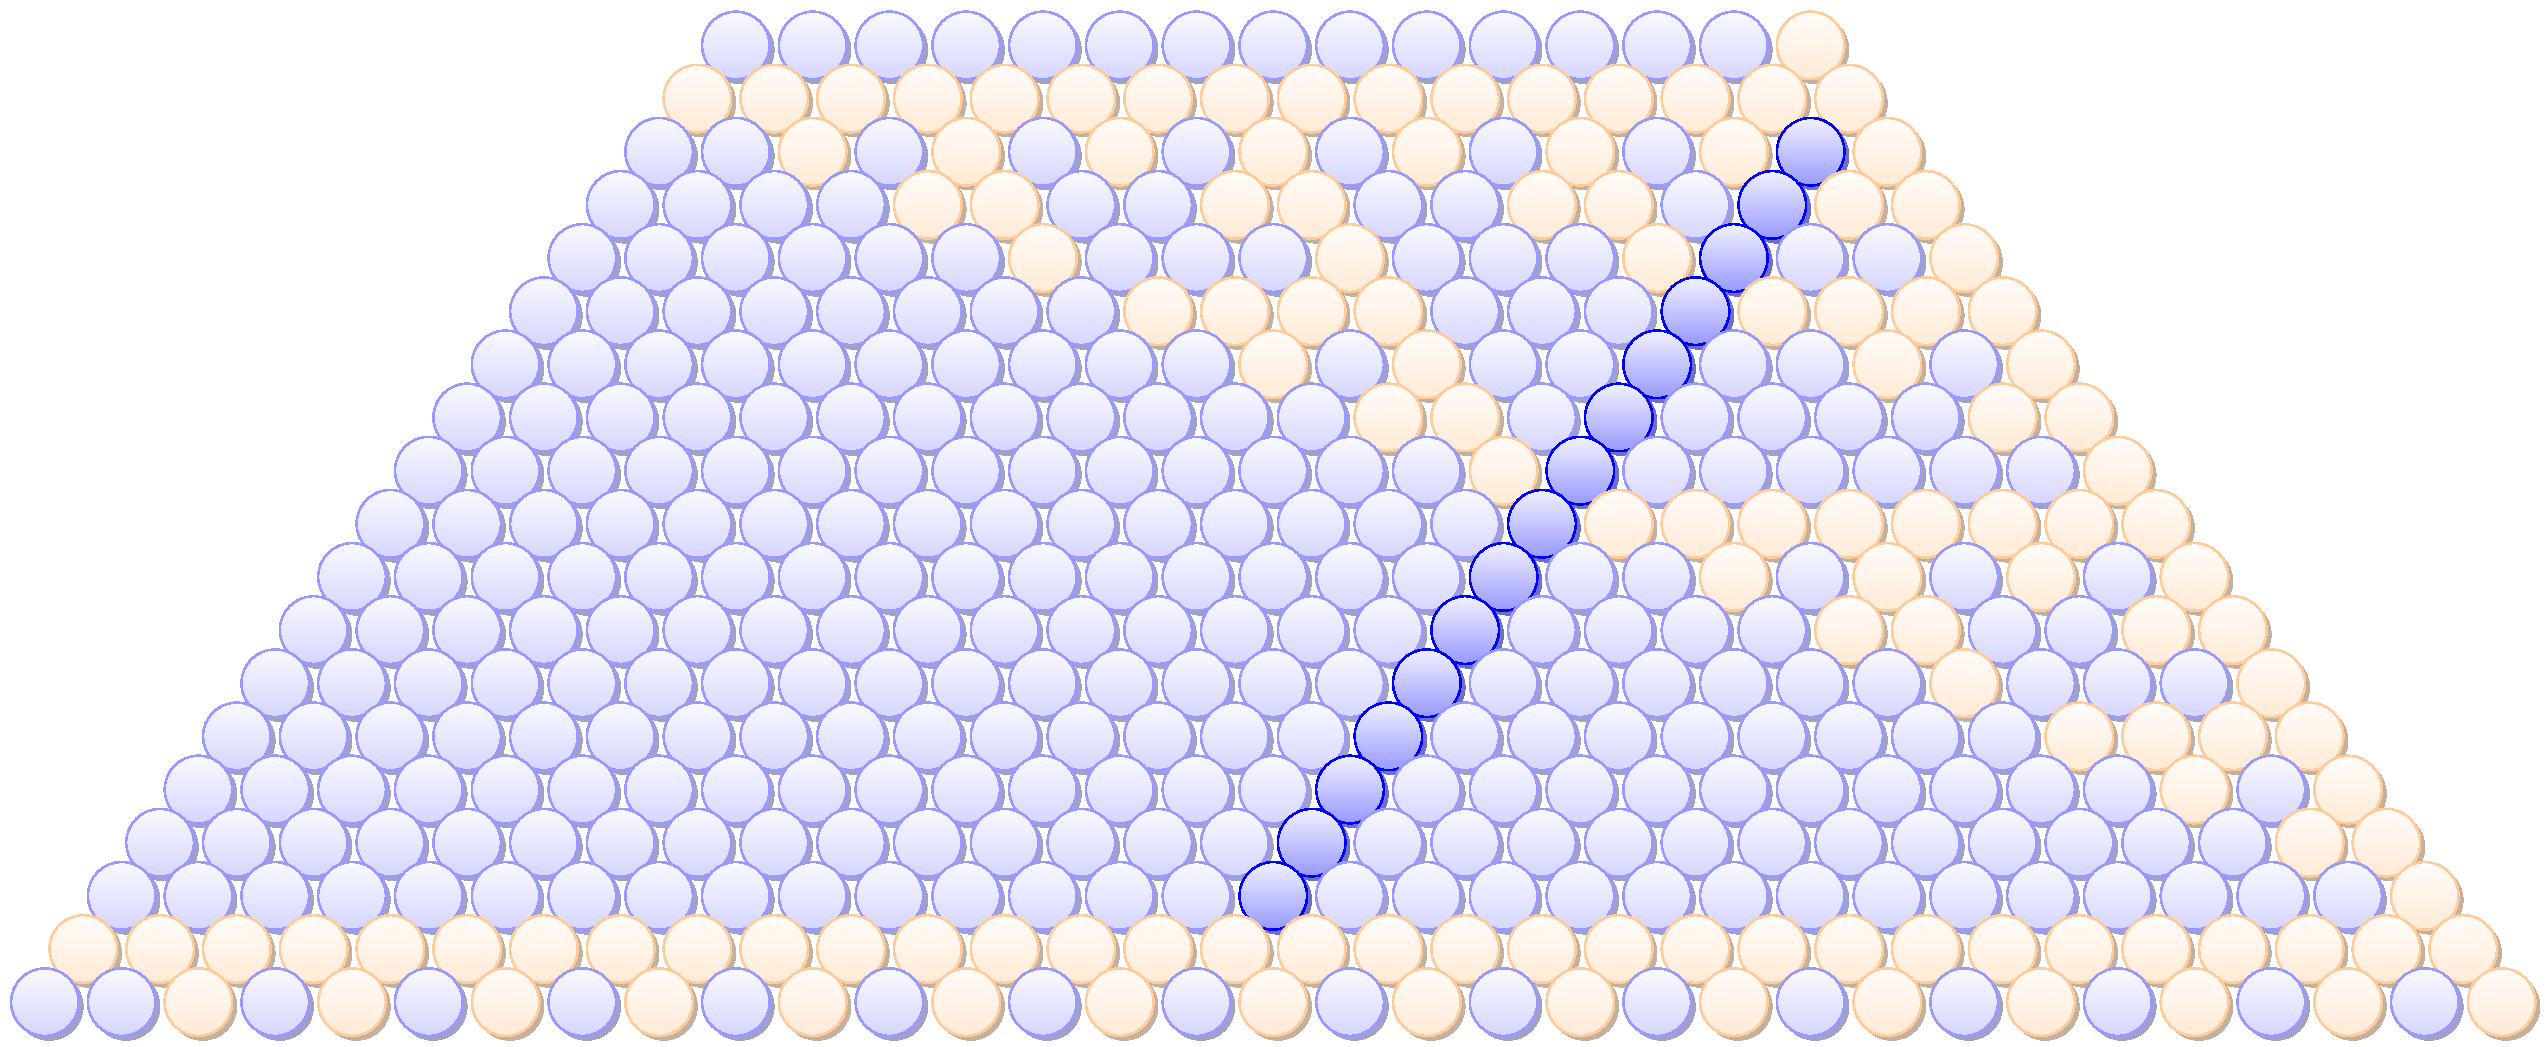
\includegraphics[width=10cm, height=10cm, keepaspectratio=true]
            {../RART2015/catalan-tikz/mirror-segment/mirror-segment.pdf}
    }

    % this 'particular' line is necessary to use `displaymath' environment
    % into the caption environment, togheter with the inclusion of 
    % `caption' package. See here for more explanation:
    % http://stackoverflow.com/questions/2716227/adding-an-equation-or-formula-to-a-figure-caption-in-latex
    \captionsetup{singlelinecheck=off}
    \caption[\emph{Mirror} segment $\Phi^{(4)}$ in $\mathcal{C}_{\equiv_{2}}^{(5)}$]
        {\emph{Mirror} segment $\Phi^{(4)}=\diagup_{\lbrace 1,2,\ldots,2^{4}-1\rbrace}^{2^{4}-1}$
        in $\mathcal{C}_{\equiv_{2}}^{(5)}$ }

    \label{fig:mirror-segment}

\end{figure}

In \autoref{fig:mirror-segment} the \emph{mirror} segment $\Phi^{(4)}$ is highlighted.

\subsection{On the \emph{dual} segment of the \emph{mirror} segment}

Next theorem needs a new piece of notation that allows us to identify a
new portion within a principal cluster $\mathcal{C}^{(\alpha+1)}$.
Let $\hat{\Phi}^{(\alpha)}$ denote the set $\left\lbrace d_{s,s-(2^{\alpha}-1)}\right\rbrace$,
for $s\in rows\left(\Phi^{(\alpha)}\right)$: we call $\hat{\Phi}^{(\alpha)}$
the \emph{dual} segment of the \emph{mirror} segment $\Phi^{(\alpha)}$.

\begin{theorem}
    Let  $\Phi^{(\alpha)}=\diagup_{\lbrace 1,2,\ldots,2^{\alpha}-1\rbrace}^{2^{\alpha}-1}$,
    be a \emph{mirror} segment in $\mathcal{C}^{(\alpha+1)}$, then:
    \begin{equation}
        d_{s,2^{\alpha}-1}\in\Phi^{(\alpha)}\rightarrow d_{s,s-(2^{\alpha}-1)}\equiv_{2}d_{s,2^{\alpha}-1}
    \end{equation}
    where $s\in rows\left(\Phi^{(\alpha)}\right)=\lbrace2^{\alpha},\ldots,2^{\alpha+1}-2\rbrace$.
\end{theorem}

\begin{proof}
    Use \autoref{eq:catalan:array:second:identity} on both members:
    \begin{displaymath}
        {{s+2^{\alpha}-1}\choose{2^{\alpha}-1}}- {{s+2^{\alpha}-1}\choose{2^{\alpha}-2}} \equiv_{2}
        {{2s-2^{\alpha}+1}\choose{s-2^{\alpha}+1}}- {{2s-2^{\alpha}+1}\choose{s-2^{\alpha}}}
    \end{displaymath}
    by symmetry property of binomial coefficients:
    \begin{displaymath}
        {{s+2^{\alpha}-1}\choose{s}}- {{s+2^{\alpha}-1}\choose{s+1}} \equiv_{2}
        {{2s-2^{\alpha}+1}\choose{s}}- {{2s-2^{\alpha}+1}\choose{s+1}}
    \end{displaymath}
    by simplification using $(-1)^{-1}\mod 2=1$:
    \begin{displaymath}
        {{s+2^{\alpha}-1}\choose{s}}+ {{s+2^{\alpha}-1}\choose{s+1}} \equiv_{2}
        {{2s-2^{\alpha}+1}\choose{s}}+ {{2s-2^{\alpha}+1}\choose{s+1}}
    \end{displaymath}
    by classic recurrence rule of binomial coefficients:
    \begin{displaymath}
        {{s+2^{\alpha}}\choose{s+1}} \equiv_{2} {{2s-2^{\alpha}+2}\choose{s+1}}
    \end{displaymath}
    since $s$ can assume $2^{\alpha}$ at least and $2^{\alpha+1}-2$ at most,
    $s$ can be written in base $2$ as follows:
    \begin{displaymath}
        s=s_{0} + s_{1}2 + s_{2}2^{2}+\ldots+s_{\alpha-1}2^{\alpha-1}+2^{\alpha}
    \end{displaymath}
    and applying Lucas theorem we get:
    \begin{displaymath}
        %\hspace{-2cm}
        {{s_{0}}\choose{s_{0}+1}}
        {{s_{1}}\choose{s_{1}}}
        \ldots
        {{s_{\alpha-1}}\choose{s_{\alpha-1}}}
        {{0}\choose{1}}
        {{1}\choose{0}}
        \equiv_{2}
        {{0}\choose{s_{0}+1}}
        {{s_{0}+1}\choose{s_{1}}}
        {{s_{1}}\choose{s_{2}}}
        \ldots
        {{s_{\alpha-2}}\choose{s_{\alpha-1}}}
        {{s_{\alpha-1}-1}\choose{1}}
        {{1}\choose{0}}
    \end{displaymath}
    simple algebra:
    \begin{displaymath}
        0
        \equiv_{2}
        {{0}\choose{s_{0}+1}}
        {{s_{0}+1}\choose{s_{1}}}
        {{s_{1}}\choose{s_{2}}}
        \ldots
        {{s_{\alpha-2}}\choose{s_{\alpha-1}}}
        {{s_{\alpha-1}-1}\choose{1}}
    \end{displaymath}
    %\marginpar{in order to finish this proof we have to introduce a lemma about
    %    the row of alternating odd and even coefficient, which can be proved using
    %    the $A$-sequence of $\mathcal{C}$}
    By cases on the parity of $s$:
    \begin{itemize}
        \item assume $s$ is \emph{even}, therefore $s_{0}=0$ and the right hand side vanishes due to ${{0}\choose{s_{0}+1}}=0$;
        \item assume $s$ is \emph{odd}, therefore $s_{0}=1$, so apply Lucas theorem to ${{0}\choose{2}}$ again,
            yielding ${{0}\choose{2}}\equiv_{2}{{0}\choose{0}}{{0}\choose{1}}\equiv_{2}0$.
    \end{itemize}
    both cases shows that right hand side is a multiple of $p$, as required.
\end{proof}


\begin{figure}[p]

    \noindent\makebox[\textwidth]{
        \centering
        %\includegraphics[width=0.8\textwidth]{../../sympy/catalan/coloured.pdf}

        % using *angle* property to rotate it is difficult to properly align it
        % in order to have a "real" matrix representation.
        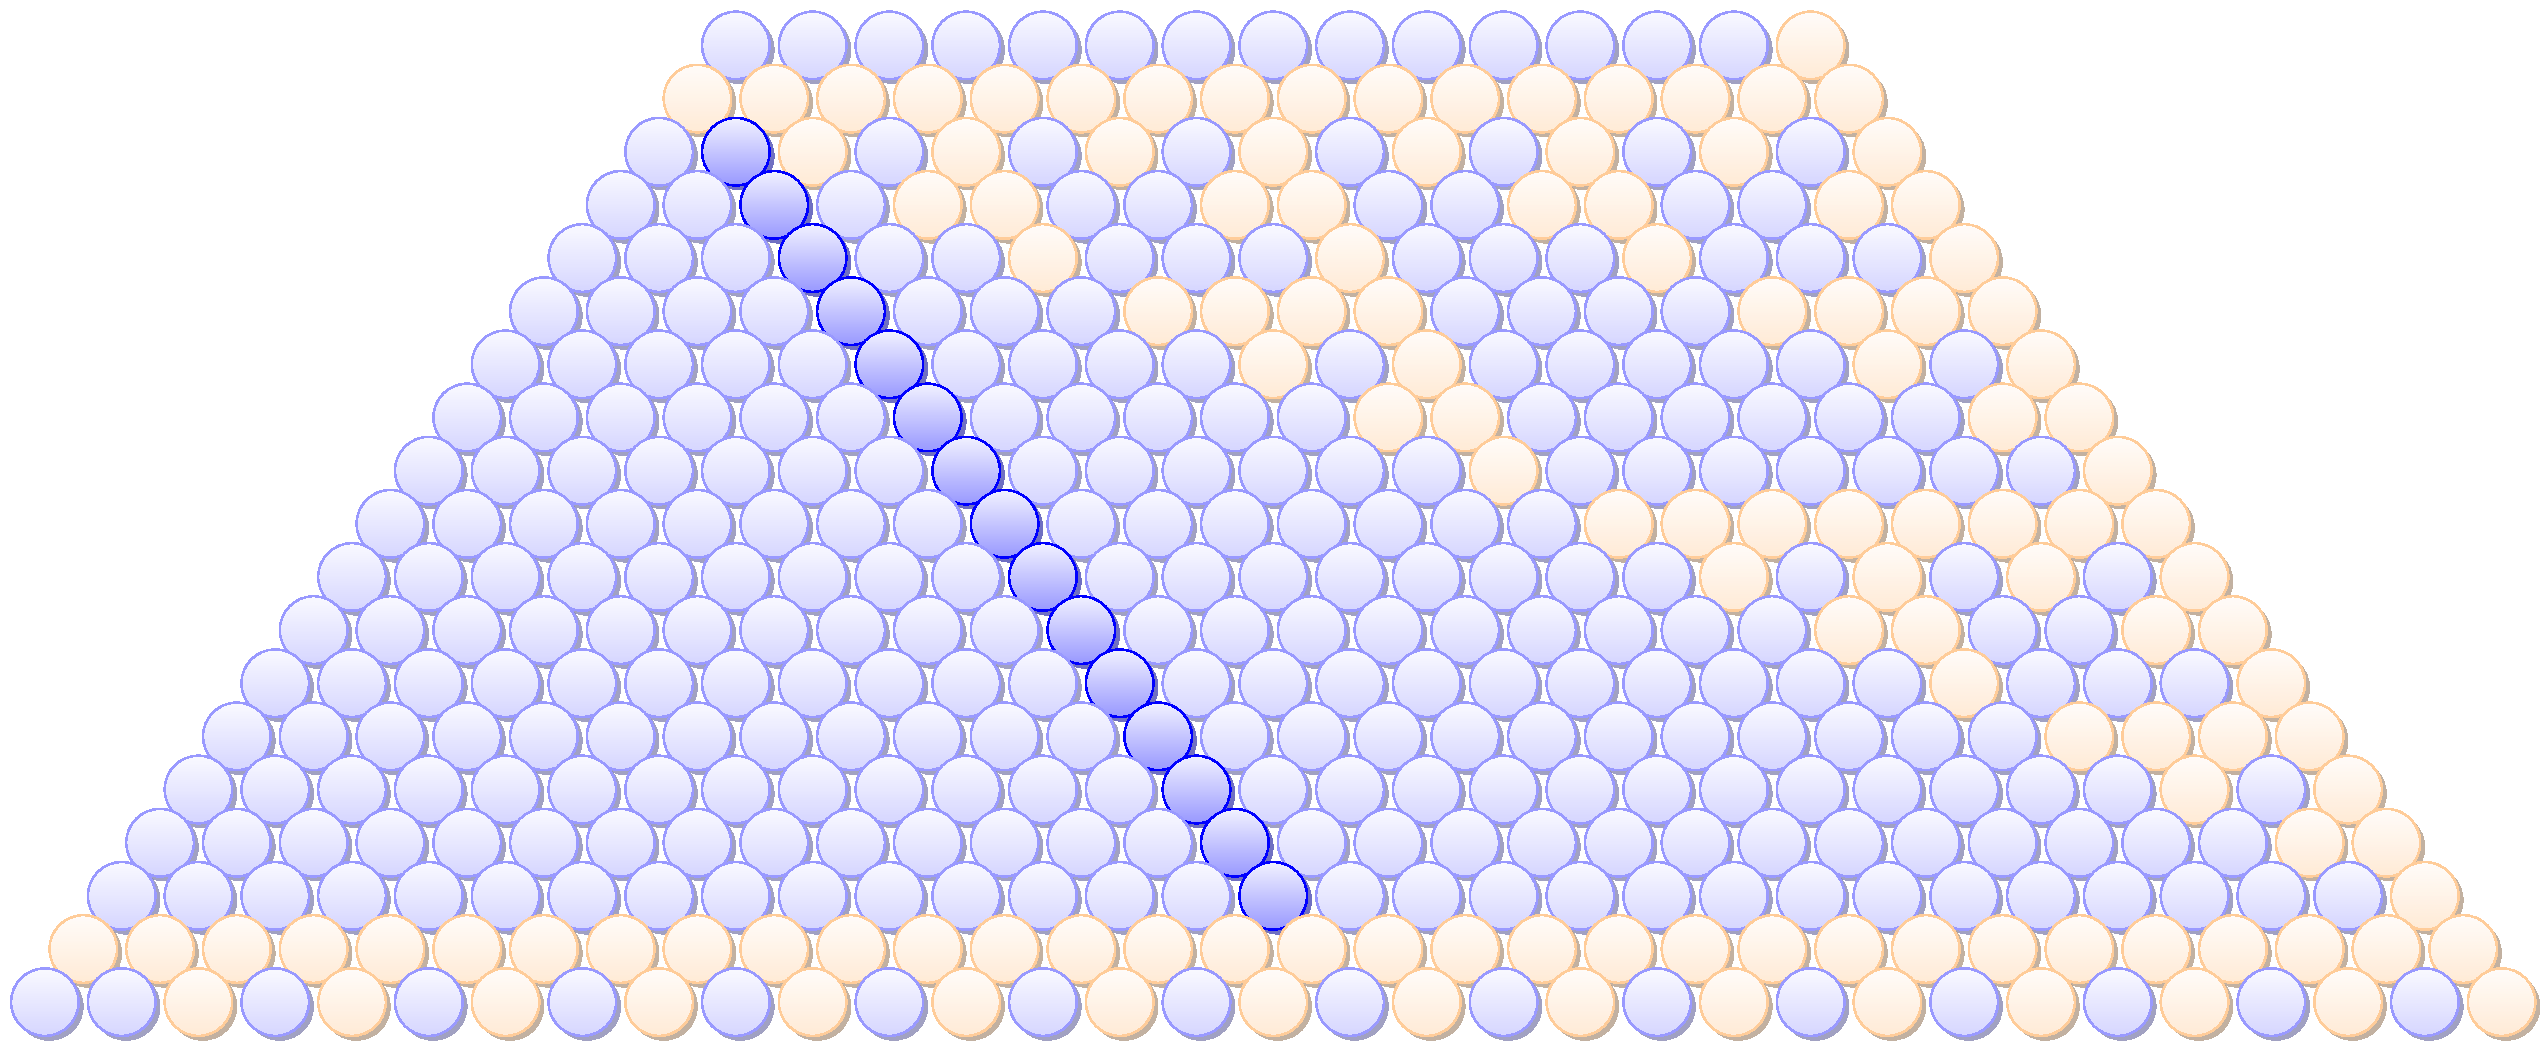
\includegraphics[width=10cm, height=10cm, keepaspectratio=true]
            {../RART2015/catalan-tikz/dual-of-mirror-segment/dual-of-mirror-segment.pdf}
    }

    % this 'particular' line is necessary to use `displaymath' environment
    % into the caption environment, togheter with the inclusion of 
    % `caption' package. See here for more explanation:
    % http://stackoverflow.com/questions/2716227/adding-an-equation-or-formula-to-a-figure-caption-in-latex
    \captionsetup{singlelinecheck=off}
    \caption[\emph{Dual} segment $\left\lbrace d_{s,s-(2^{4}-1)}\right\rbrace$,
        for $s\in rows\left(\Phi^{(4)}\right)$, in $\mathcal{C}_{\equiv_{2}}^{(5)}$]
        { \emph{Dual} segment $\left\lbrace d_{s,s-(2^{4}-1)}\right\rbrace$,
                for $s\in rows\left(\Phi^{(4)}\right)$, of \emph{mirror} segment $\Phi^{(4)}$ }



    \label{fig:dual-of-mirror-segment}

\end{figure}

In \autoref{fig:dual-of-mirror-segment} the \emph{dual} segment $\hat{\Phi}^{(4)}$
    %$\left\lbrace d_{s,s-(2^{4}-1)}\right\rbrace$,
    %for $s\in rows\left(\Phi^{(4)}\right)$,
    of \emph{mirror} segment $\Phi^{(4)}$, within $\mathcal{C}_{\equiv_{2}}^{(5)}$, is highlighted.

\subsection{On the \emph{upside-down} zero-hole}

\begin{theorem}
    Let $\mathcal{C}_{\equiv_{2}}^{(\alpha+1)}$ be a principal cluster
    of order $\alpha+1$ of the Catalan array $\mathcal{C}$. Then, $\mathcal{C}_{\equiv_{2}}^{(\alpha+1)}$
    contains an \emph{upside-down} zero-hole of order $\alpha$, denoted by $H_{\bigtriangleup}^{({\alpha})}$,
    such that coefficient $d_{n,k}\in H_{\bigtriangleup}^{({\alpha})}$ if
    $n\in\lbrace 2^{{\alpha}},\ldots,2^{{\alpha}+1}-2\rbrace$ and
    $k\in\lbrace 0,\ldots, n-2^{{\alpha}}\rbrace$.
    \label{thm:upside:down:zero:hole}
\end{theorem}

%It is simple to observe that $H_{\bigtriangleup}^{({\alpha})}\subset \mathcal{C}_{\equiv_{2}}^{(\alpha+1)}$.

\begin{proof}
We repeatedly use the approach
of the proof about the \emph{mirror} segment, considering the set of columns
$\Xi=\lbrace \vect{c}_{0},\ldots, \vect{c}_{2^{{\alpha}}-2}\rbrace$ and
for each column $\vect{c}_{k}\in\Xi$, the segment
    $\diagup_{\lbrace 2^{\alpha},2^{\alpha}+1,\ldots,2^{\alpha+1}-2-k\rbrace}^{k}$.

If we start from the column $\vect{c}_{0}$ on the very left,
then the corresponding set of row indices is a segment of Catalan numbers:
\begin{displaymath}
    S_{0}=\diagup_{\lbrace 2^{\alpha},2^{\alpha}+1,\ldots,2^{\alpha+1}-2\rbrace}^{0}
        = \lbrace C_{2^{\alpha}},C_{2^{\alpha}+1},\ldots,C_{2^{\alpha+1}-2}\rbrace
\end{displaymath}
since no coefficient $C_{j}\in S_{0}$ has the shape $C_{2^{\alpha}-1}$,
all coefficients in $S_{0}$ are even.

In turn, take into account column $\vect{c}_{1}$, so the corresponding segment is
%\begin{displaymath}
    $S_{1}=\diagup_{\lbrace 2^{\alpha},2^{\alpha}+1,\ldots,2^{\alpha+1}-3\rbrace}^{1}$
    %S_{1}=\lbrace d_{2^{{\alpha}}+1,1},\ldots,d_{2^{{\alpha}+1}-2,1} \rbrace
%\end{displaymath}
and coefficients in it are defined according to
$d_{s, 1} = \sum_{i_{1}+i_{2}=s+1} {C_{i_{1}-1}\,C_{i_{2}-1}}$,
where $s\in rows(S_{1})= \left\lbrace 2^{\alpha}+1,2^{\alpha}+2,\ldots,2^{\alpha+1}-2\right\rbrace$.
This is quite similar to the proof developed for the \emph{mirror} segment,
with the difference that summand term is composed of two coefficients, namely
$C_{i_{1}-1}\,C_{i_{2}-1}$ instead of $2^{{\alpha}}$ coefficients as in the previous proof,
therefore the same argument applies,
since if multiplying $2^{{\alpha}}$ coefficients fails to make \emph{not} vanish
the summand term, modulo $2$, the same failure is reached if multiplying only $2$ coefficients.

The same reasoning holds for remaining columns in $\Xi$: the last one of them is
$\vect{c}_{2^{\alpha}-2}$ (with only \emph{one} coefficient, namely $d_{2^{\alpha}-2,2^{\alpha}-2}$),
hence $H_{\bigtriangleup}^{({\alpha})}$ is an \emph{upside-down} zero-holes of order $\alpha$,
positioned at the very left in the bottom half of $\mathcal{C}_{\equiv_{2}}^{(\alpha+1)}$, as required.

\end{proof}


\begin{figure}[p]

    \noindent\makebox[\textwidth]{
        \centering
        %\includegraphics[width=0.8\textwidth]{../../sympy/catalan/coloured.pdf}

        % using *angle* property to rotate it is difficult to properly align it
        % in order to have a "real" matrix representation.
        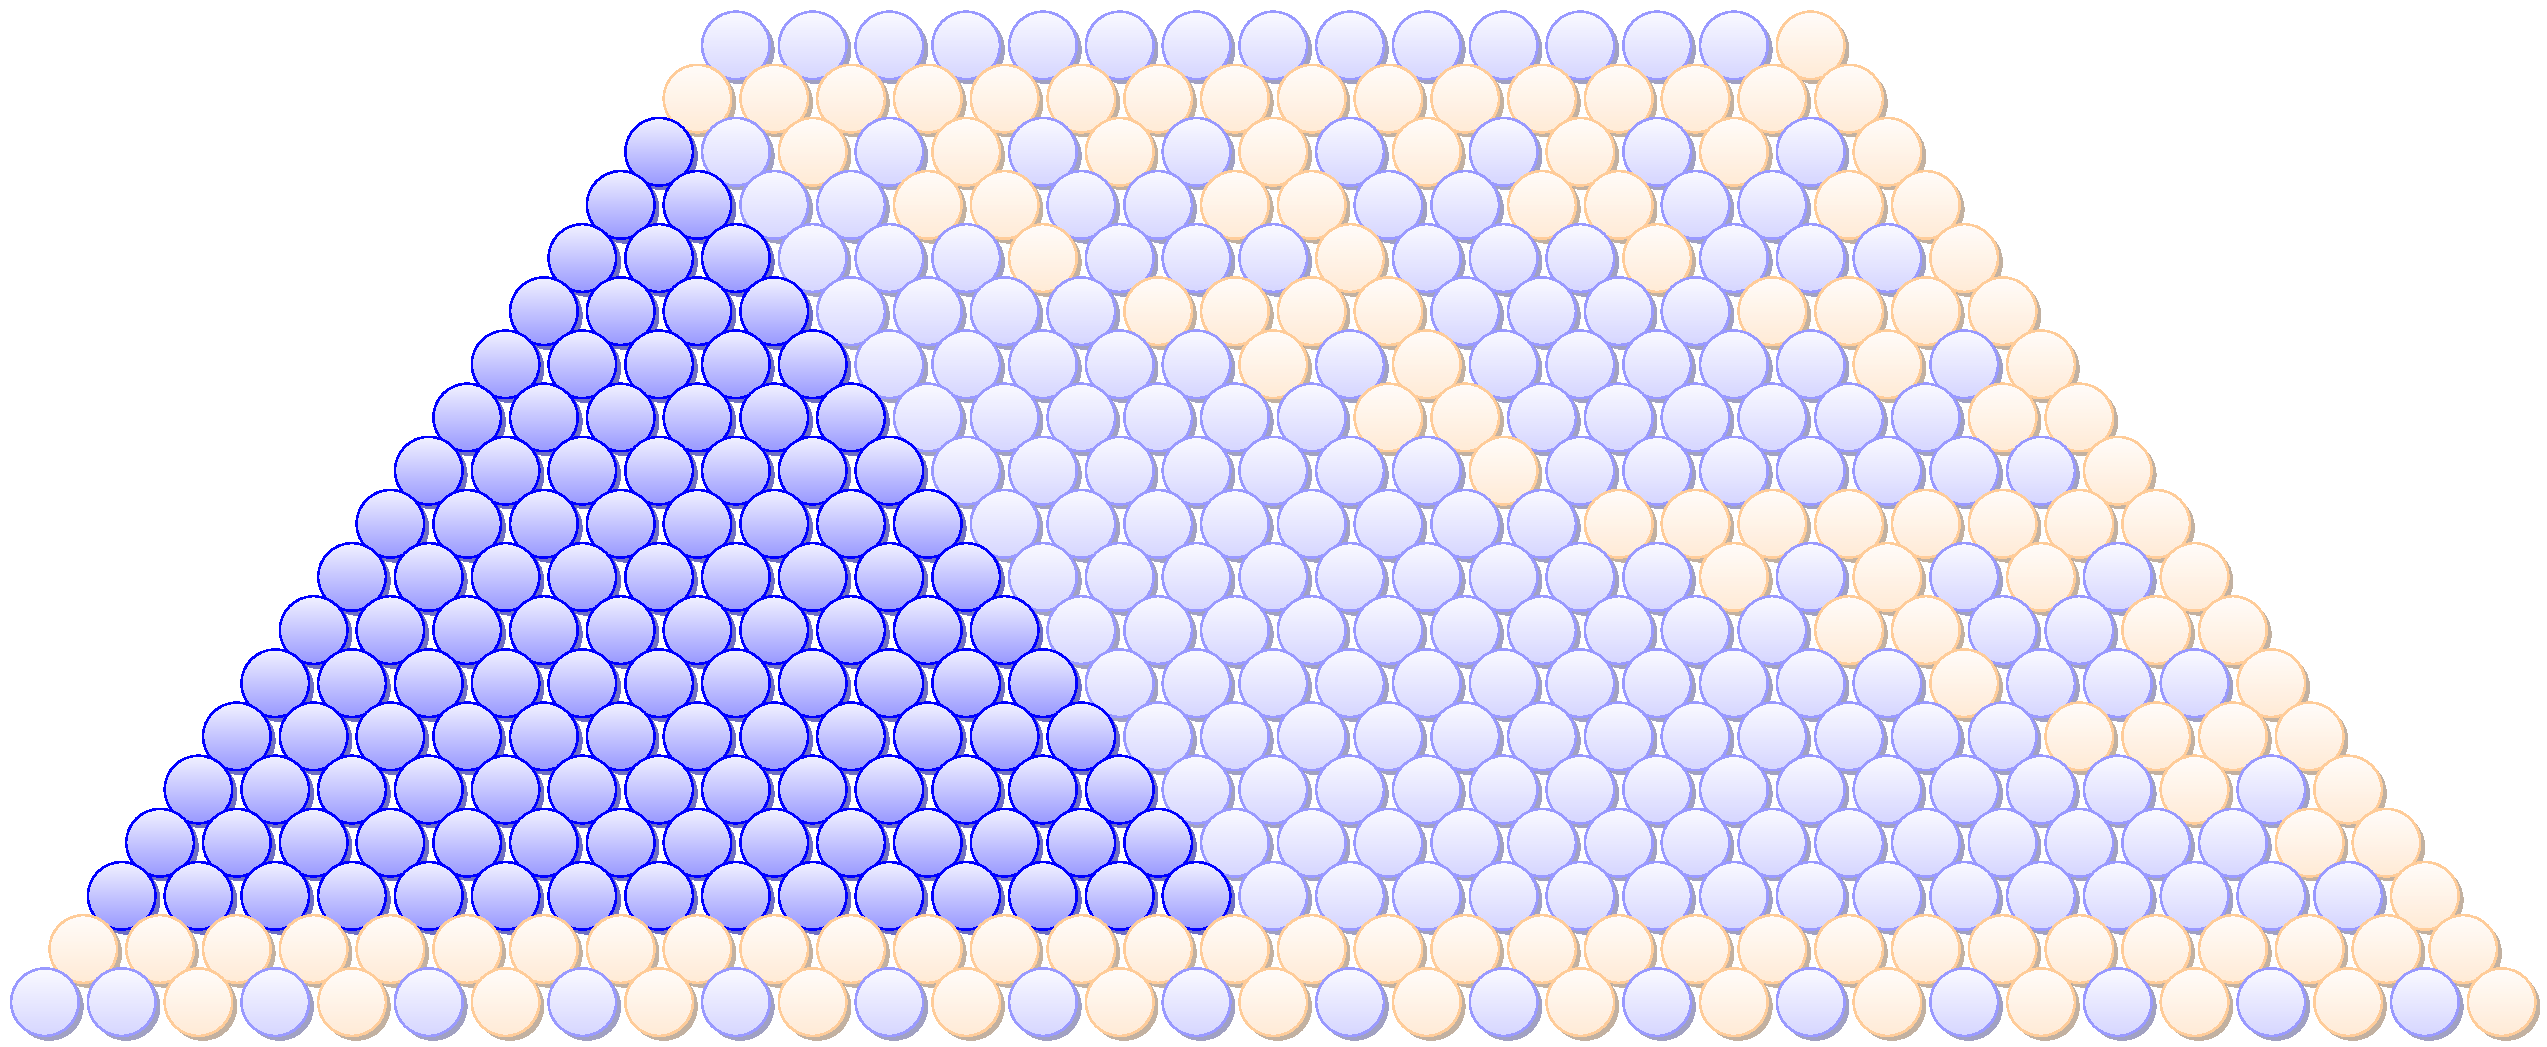
\includegraphics[width=10cm, height=10cm, keepaspectratio=true]
            {../RART2015/catalan-tikz/zero-hole/zero-hole.pdf}
    }

    % this 'particular' line is necessary to use `displaymath' environment
    % into the caption environment, togheter with the inclusion of 
    % `caption' package. See here for more explanation:
    % http://stackoverflow.com/questions/2716227/adding-an-equation-or-formula-to-a-figure-caption-in-latex
    \captionsetup{singlelinecheck=off}
    \caption[Upside-down zero-hole $T_{\bigtriangleup}^{(4)}$ within
        $\mathcal{C}_{\equiv_{2}}^{(\alpha+1)}$]{Zero hole $T_{\bigtriangleup}^{(4)} \subset \mathcal{C}_{\equiv_{2}}^{(5)}$}

    \label{fig:catalan-zero-hole}

\end{figure}

In \autoref{fig:catalan-zero-hole} is reported $H_{\bigtriangleup}^{(4)}$.

\subsection{On two \emph{mirrored} clusters}

\begin{theorem}
    Let $\Phi^{(\alpha)}=\diagup_{\lbrace 2,\ldots,2^{\alpha}-1\rbrace}^{2^{\alpha}-1}$
    be a \emph{mirror} segment and $d_{s,2^{{\alpha}}-1}$
    be a coefficient in $\Phi^{(\alpha)}$, for some $s\in rows\left(\Phi^{(\alpha)}\right)$. Then:
    \begin{displaymath}
        d_{s-e,2^{{\alpha}}-1-e} \equiv_{2} d_{s,2^{{\alpha}}-1+e}
    \end{displaymath}
    for $e\in\lbrace1,\ldots,s-2^{{\alpha}}\rbrace$.
    \label{thm:two:mirrored:clusters}
\end{theorem}

\begin{proof}
In this proof we use \autoref{eq:catalan:array:second:identity} as
an identity defining the generic coefficient. It allows to rewrite the left hand side
of the argument:
\begin{displaymath}
    d_{s-e,2^{{\alpha}}-1-e}= {{2(s-e)-(2^{{\alpha}}-1-e)}\choose{(s-e)-(2^{{\alpha}}-1-e)}}
        - {{2(s-e)-(2^{{\alpha}}-1-e)}\choose{(s-e)-(2^{{\alpha}}-1-e)-1}};
\end{displaymath}
in the same spirit, the same can be applied to the right hand side:
\begin{displaymath}
    d_{s,2^{{\alpha}}-1+e}={{2s-(2^{{\alpha}}-1+e)}\choose{s-(2^{{\alpha}}-1+e)}}
        - {{2s-(2^{{\alpha}}-1+e)}\choose{s-(2^{{\alpha}}-1+e)-1}},
\end{displaymath}
therefore:
\begin{displaymath}
    \begin{split}
        {{2s-e-2^{{\alpha}}+1}\choose{s-2^{{\alpha}}+1}}
            - {{2s-e-2^{{\alpha}}+1}\choose{s-2^{{\alpha}}}}
        &\equiv_{2}
        {{2s-2^{{\alpha}}+1-e}\choose{s-2^{{\alpha}}+1-e}}
            - {{2s-2^{{\alpha}}+1-e}\choose{s-2^{{\alpha}}-e}}\\
        {{2s-e-2^{{\alpha}}+1}\choose{s-e}}
            - {{2s-e-2^{{\alpha}}+1}\choose{s-e+1}}
        &\equiv_{2}
        {{2s-2^{{\alpha}}+1-e}\choose{s}}
            - {{2s-2^{{\alpha}}+1-e}\choose{s+1}}\\
    \end{split}
\end{displaymath}

Since $e\in\lbrace1,\ldots,s-2^{{\alpha}}\rbrace$, proceed by complete induction on $e$:
\begin{itemize}
    \item base case $e=1$ yield the following congruence:
        \begin{displaymath}
                {{2s-2^{{\alpha}}}\choose{s-1}}-{{2s-2^{{\alpha}}}\choose{s}}
                \equiv_{2}
                {{2s-2^{{\alpha}}}\choose{s}}-{{2s-2^{{\alpha}}}\choose{s+1}}\\
        \end{displaymath}
        which is the same to say:
        \begin{displaymath}
                {{2s-2^{{\alpha}}}\choose{s-1}}+{{2s-2^{{\alpha}}}\choose{s+1}} \equiv_{2} 0.
        \end{displaymath}
        Let $s=s_{0}+s_{1}\,2+s_{2}\,2^{2}+\ldots+s_{{\alpha}-1}\,2^{{\alpha}-1} + 2^{{\alpha}}$
        be the generic representation of $s$ in base $2$, since
        $s\in\lbrace 2^{{\alpha}}+1,\ldots,2^{{\alpha}+1}-2 \rbrace$; also
        let $2s-2^{{\alpha}}=s_{0}\,2+s_{1}\,2^{2}+s_{2}\,2^{3}+\ldots+s_{{\alpha}-1}^{*}\,2^{{\alpha}} + s_{{\alpha}}^{*}\,2^{{\alpha}+1}$,
        where $(s_{{\alpha}-1}^{*},s_{{\alpha}}^{*})$ equals $(0,1)$ if $s_{{\alpha}-1}=1$, otherwise equals $(1,0)$.
        By cases on the parity of $s$:
        \begin{itemize}
            \item assume $s$ even, therefore both $s-1$ and $s+1$ are odd, so
                let $\hat{s}=1+\hat{s}_{1}\,2+\hat{s}_{2}\,2^{2}+\ldots+
                    \hat{s}_{{\alpha}-1}\,2^{{\alpha}-1}+2^{{\alpha}}$ be one of them, hence:
                \begin{displaymath}
                        {{2s-2^{{\alpha}}}\choose{\hat{s}}}
                        \equiv_{2}
                        {{0}\choose{1}}
                        {{0}\choose{\hat{s}_{1}}}
                        {{s_{1}}\choose{\hat{s}_{2}}}
                        \ldots
                        {{s_{{\alpha}-2}}\choose{\hat{s}_{{\alpha}-1}}}
                        {{s_{{\alpha}-1}^{*}}\choose{1}}
                        {{s_{{\alpha}}^{*}}\choose{0}} = 0.
                \end{displaymath}
                Observe $\hat{s}_{{\alpha}}=1$ against boundary cases:
                if $s=2^{{\alpha}}+1$ then $\hat{s}=s-1=2^{{\alpha}}$, on the other
                hand if $s=2^{{\alpha}+1}-2$ then $\hat{s}=s+1=2^{{\alpha}+1}-1$,
                therefore in both cases the coefficient of $2^{{\alpha}}$ is $1$.
                Eventually we get $0+0 \equiv_{2}0$, which holds;

            \item assume $s$ odd, therefore both $s-1$ and $s+1$ are even,
                let's study the former:
                \begin{displaymath}
                        {{2s-2^{{\alpha}}}\choose{s-1}}
                        \equiv_{2}
                        {{0}\choose{0}}
                        {{1}\choose{s_{1}}}
                        {{s_{1}}\choose{s_{2}}}
                        \ldots
                        {{s_{{\alpha}-2}}\choose{s_{{\alpha}-1}}}
                        {{s_{{\alpha}-1}^{*}}\choose{1}}
                        {{s_{{\alpha}}^{*}}\choose{0}}
                \end{displaymath}
                in order for the right hand side to not vanish, modulo $2$,
                it is mandatory for coefficients $\lbrace s_{i}\rbrace_{i\in\lbrace1,\ldots,{\alpha}-2\rbrace}$
                to satisfy $s_{i}\geq s_{i+1}$: if any one of them is $0$, say $s_{j}$, then
                $s_{j+1},\ldots,s_{j+k}$, with $j+k={\alpha}-1$,
                have to be all $0$ too. In particular, if $s_{{\alpha}-1}=0$ then
                $(s_{{\alpha}-1}^{*},s_{{\alpha}}^{*})=(1,0)$
                therefore the right hand side reduces to $1$, modulo $2$.
                Observe that coefficients $\lbrace s_{i}\rbrace_{i\in\lbrace1,\ldots,{\alpha}-2\rbrace}$
                cannot be all $1$ otherwise
                $s=(\underbrace{1,1,1,\ldots,1}_{{\alpha}+1})_{2}=2^{{\alpha}+1}-1$ raises a contradiction, because
                $s$ can assume $2^{{\alpha}+1}-2$ at most.

                For the latter, namely $s+1$, assume $s$ can be represented as:
                \begin{displaymath}
                    (\underbrace{1,1,\ldots,1}_{r},0,s_{r+1},s_{r+2},\ldots,s_{{\alpha}-1},1)_{2}
                \end{displaymath}
                for $r\in\lbrace1,\ldots,{\alpha}-2\rbrace$. Since a $0$ must occur, otherwise $s=2^{{\alpha}+1}-1$
                which cannot be the case as we've already seen, adding $1$ yield the representation:
                \begin{displaymath}
                    (\underbrace{0,0,\ldots,0}_{r},1,s_{r+1},s_{r+2},\ldots,s_{{\alpha}-1},1)_{2}
                \end{displaymath}
                Therefore we have:
                \begin{displaymath}
                    %\hspace{-2cm}
                    {{2s-2^{{\alpha}}}\choose{s+1}}
                    \equiv_{2}
                    \underbrace{
                        {{0}\choose{0}}
                        {{1}\choose{0}}
                        {{1}\choose{0}}
                        \ldots
                        {{1}\choose{0}}
                    }_{r}
                    {{1}\choose{1}}
                    {{0}\choose{s_{r+1}}}
                    {{s_{r+1}}\choose{s_{r+2}}}
                    \ldots
                    {{s_{{\alpha}-2}}\choose{s_{{\alpha}-1}}}
                    {{s_{{\alpha}-1}^{*}}\choose{1}}
                    {{s_{{\alpha}}^{*}}\choose{0}}
                \end{displaymath}
                In order to not vanish, modulo $2$,
                $s_{r+1}$ has to be $0$; eventually, this property propagates among $s_{r+2}, \ldots, s_{{\alpha}-1}$.
                But if they are all $0$, %$s_{{\alpha}-1}=0$
                then $(s_{{\alpha}-1}^{*},s_{{\alpha}}^{*})=(1,0)$, therefore the right hand side reduces to $1$.

                Combining the above cases for $s$ odd we reach:
                \begin{displaymath}
                        {{2s-2^{{\alpha}}}\choose{s-1}}+{{2s-2^{{\alpha}}}\choose{s+1}} \equiv_{2} 1+1\equiv_{2} 0
                \end{displaymath}
        \end{itemize}

        \item assume the argument holds for $k\leq e$ and prove for $k=e+1$, so we need to show:
            \begin{displaymath}
                \footnotesize
                %\hspace{-3cm}
                \begin{split}
                    {{2s-(e+1)-2^{{\alpha}}+1}\choose{s-2^{{\alpha}}+1}}
                        - {{2s-(e+1)-2^{{\alpha}}+1}\choose{s-2^{{\alpha}}}}
                    &\equiv_{2}
                    {{2s-2^{{\alpha}}+1-(e+1)}\choose{s-2^{{\alpha}}+1-(e+1)}}
                        - {{2s-2^{{\alpha}}+1-(e+1)}\choose{s-2^{{\alpha}}-(e+1)}}\\
                    {{2s-(e+1)-2^{{\alpha}}+1}\choose{s-(e+1)}}
                        - {{2s-(e+1)-2^{{\alpha}}+1}\choose{s-(e+1)+1}}
                    &\equiv_{2}
                    {{2s-2^{{\alpha}}+1-(e+1)}\choose{s}}
                        - {{2s-2^{{\alpha}}+1-(e+1)}\choose{s+1}}\\
                    {{2s-e-2^{{\alpha}}}\choose{s-e-1}}
                        - {{2s-e-2^{{\alpha}}}\choose{s-e}}
                    &\equiv_{2}
                    {{2s-2^{{\alpha}}-e}\choose{s}}
                        - {{2s-2^{{\alpha}}-e}\choose{s+1}}\\
                \end{split}
            \end{displaymath}
            which follows directly by complete induction hypothesis.
\end{itemize}

\end{proof}


\begin{figure}[htb]

    \noindent\makebox[\textwidth]{
        \centering
        %\includegraphics[width=0.8\textwidth]{../../sympy/catalan/coloured.pdf}

        % using *angle* property to rotate it is difficult to properly align it
        % in order to have a "real" matrix representation.
        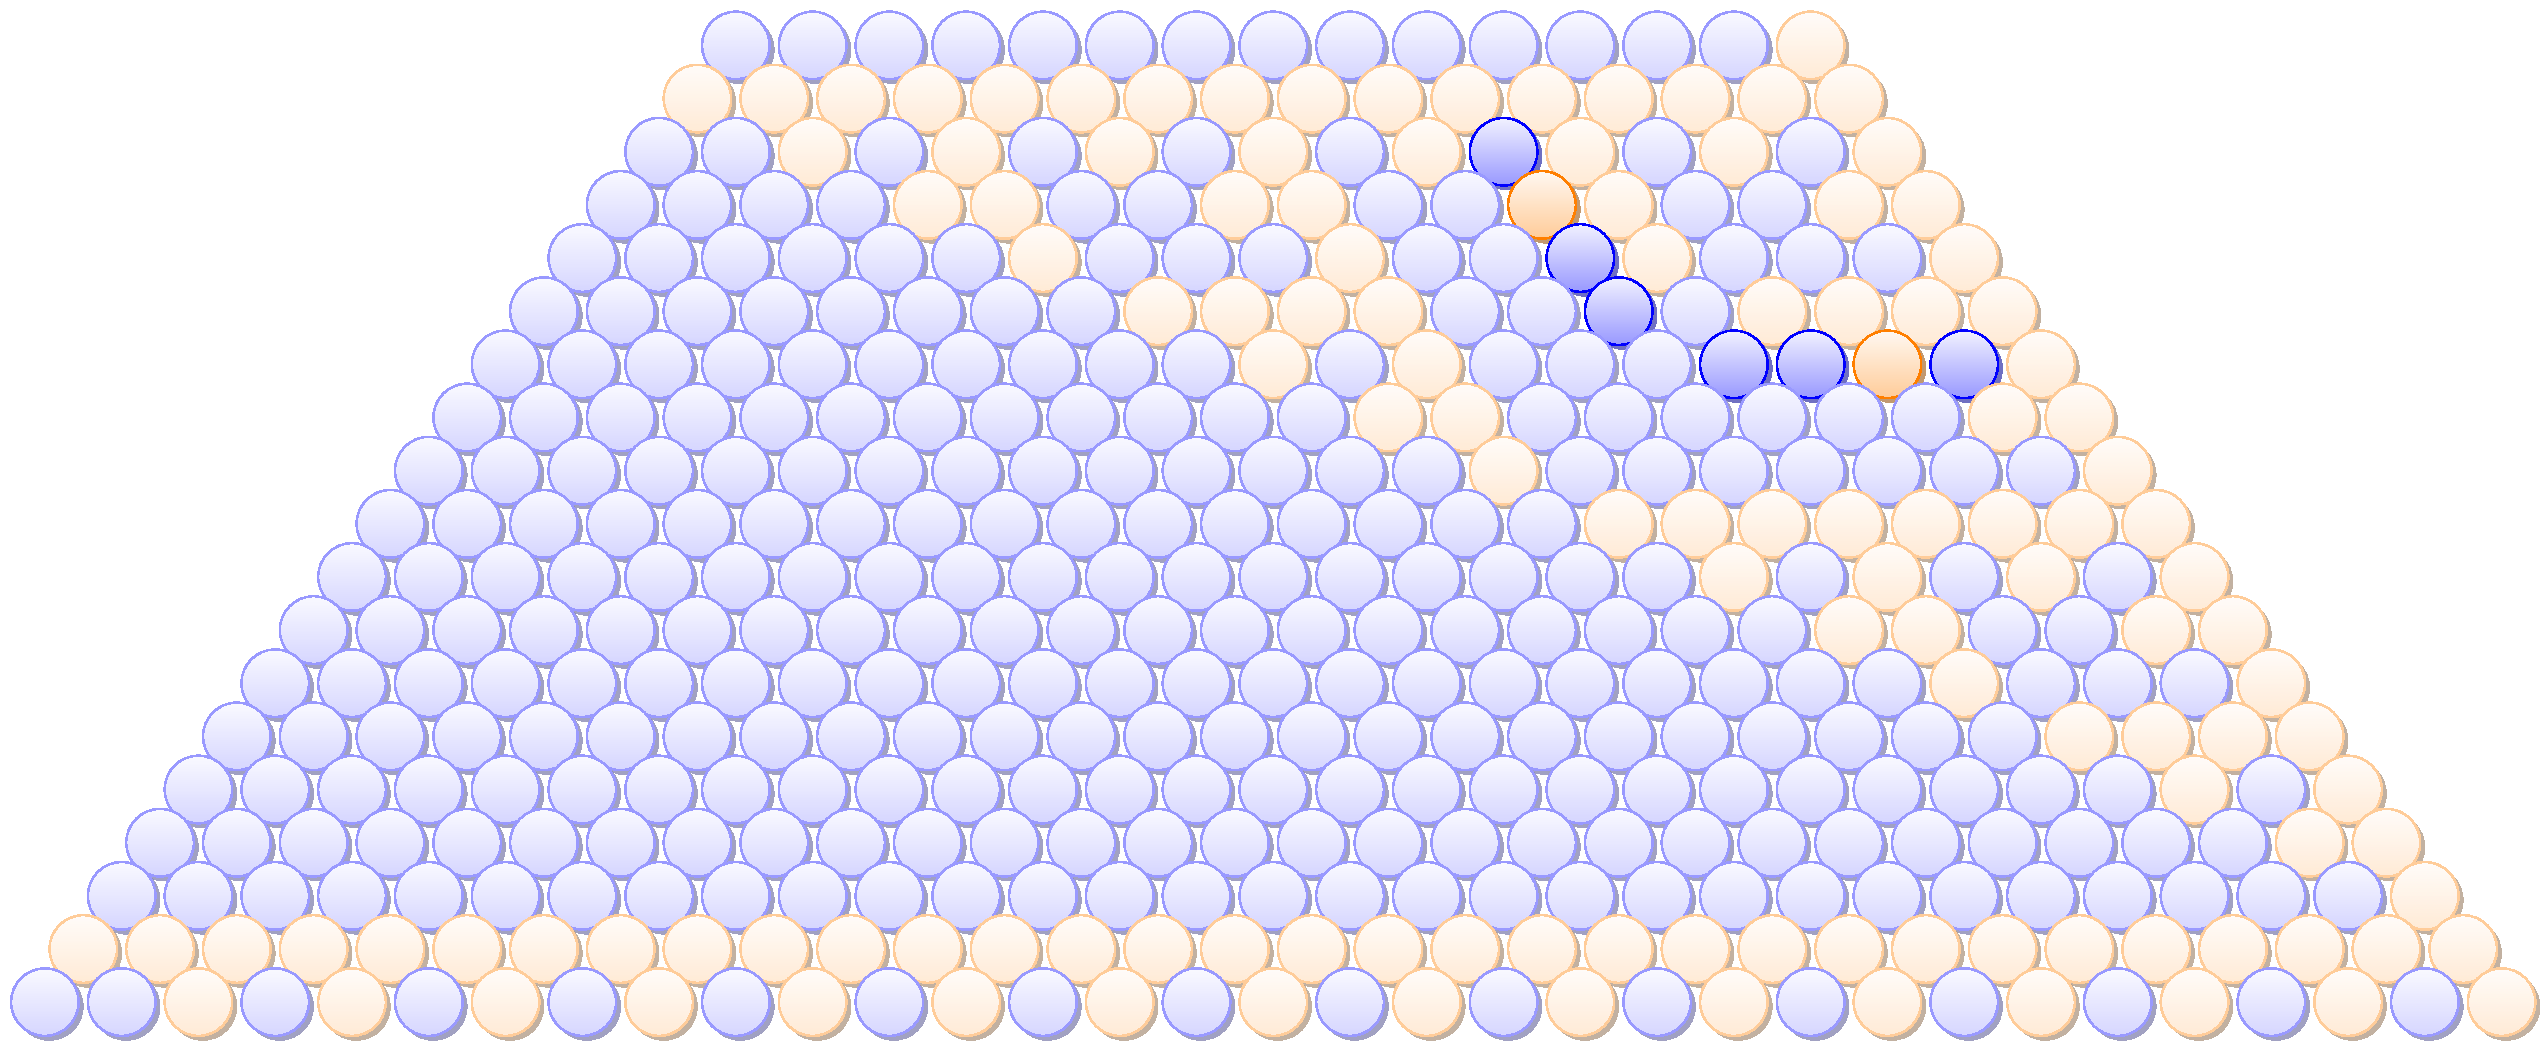
\includegraphics[width=10cm, height=10cm, keepaspectratio=true]
            {../RART2015/catalan-tikz/mirrored-clusters/mirrored-clusters.pdf}
    }

    % this 'particular' line is necessary to use `displaymath' environment
    % into the caption environment, togheter with the inclusion of 
    % `caption' package. See here for more explanation:
    % http://stackoverflow.com/questions/2716227/adding-an-equation-or-formula-to-a-figure-caption-in-latex
    \captionsetup{singlelinecheck=off}
    \caption[\emph{Mirrored} principal clusters $\mathcal{C}_{\equiv_{2}}^{(4)}$]
        {Some coefficients in \emph{mirrored} cluster $\mathcal{C}_{\equiv_{2}}^{(4)}$ 
        over $\hat{d}_{20,2^{4}-1}$: congruences $d_{20-e,2^{4}-1-e} \equiv_{2} d_{20,2^{4}-1+e}$ 
        for $e\in\lbrace1,\ldots,4\rbrace$ }

    \label{fig:catalan-mirrored-clusters}

\end{figure}

In \autoref{fig:catalan-mirrored-clusters} some coefficients in \emph{mirrored}
cluster $\mathcal{C}_{\equiv_{2}}^{(4)}$ are highlighted.

\subsection{$\mathcal{C}_{\equiv_{2}}^{(\alpha+1)}$
    contains a copy of $\mathcal{C}_{\equiv_{2}}^{(\alpha)}$}

In order to fully characterize $\mathcal{C}$ in a modular context we are
left with a last theorem.

\begin{theorem}
    $\mathcal{C}_{\equiv_{2}}^{(\alpha+1)}$
    contains a copy of $\mathcal{C}_{\equiv_{2}}^{(\alpha)}$,
    located at the very right of its bottom half. Formally,
    let $\Phi^{(\alpha)}=\diagup_{\lbrace 2,\ldots,2^{\alpha}-1\rbrace}^{2^{\alpha}-1}$
    be a \emph{mirror} segment and $d_{s,2^{{\alpha}}-1}$
    be a coefficient in $\Phi^{(\alpha)}$, for some $s\in rows\left(\Phi^{(\alpha)}\right)$. Then:
    \begin{displaymath}
        d_{s,2^{{\alpha}}-1+e} \equiv_{2} d_{s-2^{{\alpha}},e-1}
    \end{displaymath}
    for $e\in\lbrace1,\ldots,s-2^{{\alpha}}\rbrace$.
    \label{thm:principal:cluster:copy:containment}
\end{theorem}

\begin{proof}
We tackle the proof using \autoref{eq:catalan:array:second:identity}:
\begin{displaymath}
    %\hspace{-4cm}
    \begin{split}
        {{2s-(2^{{\alpha}}-1+e)}\choose{s-(2^{{\alpha}}-1+e)}} - {{2s-(2^{{\alpha}}-1+e)}\choose{s-(2^{{\alpha}}-1+e)-1}}
        &\equiv_{2}
        {{2(s-2^{{\alpha}})-(e-1)}\choose{(s-2^{{\alpha}})-(e-1)}} - {{2(s-2^{{\alpha}})-(e-1)}\choose{(s-2^{{\alpha}})-(e-1)-1}}\\
        {{2s-2^{{\alpha}}+1-e}\choose{s-2^{{\alpha}}+1-e}} - {{2s-2^{{\alpha}}+1-e}\choose{s-2^{{\alpha}}-e}}
        &\equiv_{2}
        {{2s-2^{{\alpha}+1}-e+1}\choose{s-2^{{\alpha}}-e+1}} - {{2s-2^{{\alpha}+1}-e+1}\choose{s-2^{{\alpha}}-e}}\\
        {{2s-2^{{\alpha}}+1-e}\choose{s}} - {{2s-2^{{\alpha}}+1-e}\choose{s+1}} &\equiv_{2}
        {{2s-2^{{\alpha}+1}-e+1}\choose{s-2^{{\alpha}}}} - {{2s-2^{{\alpha}+1}-e+1}\choose{s-2^{{\alpha}}+1}}\\
    \end{split}
\end{displaymath}
Since $e\in\lbrace1,\ldots,s-2^{{\alpha}}\rbrace$, proceed by complete induction on $e$:
    \begin{itemize}
        \item for the base case $e=1$ we have:
            \begin{displaymath}
                %\begin{split}
                    {{2s-2^{{\alpha}}}\choose{s}} - {{2s-2^{{\alpha}}}\choose{s+1}} \equiv_{2}
                        {{2s-2^{{\alpha}+1}}\choose{s-2^{{\alpha}}}} - {{2s-2^{{\alpha}+1}}\choose{s-2^{{\alpha}}+1}}.
                %\end{split}
            \end{displaymath}
            In the previous proof a detailed (and boring) derivation has been performed,
            here we observe that upper terms of each binomial coefficient, $2s-2^{{\alpha}}$
            and $2s-2^{{\alpha}+1}$ respectively, have $2$ in their prime factorization, therefore
            expanding each binomial, $2$ can be factored out in turn, making congruent $0$
            each one of them. However an approach similar to the previous one can be
            taken as well.

        \item assume the argument holds for $k\leq e$ and prove for $k=e+1$, so we need to show:
            \begin{displaymath}
                %\hspace{-3cm}
                \footnotesize
                \begin{split}
                    {{2s-2^{{\alpha}}+1-(e+1)}\choose{s}} - {{2s-2^{{\alpha}}+1-(e+1)}\choose{s+1}}
                    &\equiv_{2}
                    {{2s-2^{{\alpha}+1}-(e+1)+1}\choose{s-2^{{\alpha}}}} - {{2s-2^{{\alpha}+1}-(e+1)+1}\choose{s-2^{{\alpha}}+1}}\\
                    {{2s-2^{{\alpha}}-e}\choose{s}} - {{2s-2^{{\alpha}}-e}\choose{s+1}}
                    &\equiv_{2}
                    {{2s-2^{{\alpha}+1}-e}\choose{s-2^{{\alpha}}}} - {{2s-2^{{\alpha}+1}-e}\choose{s-2^{{\alpha}}+1}}\\
                \end{split}
            \end{displaymath}
            which follows directly by complete induction hypothesis.
    \end{itemize}
\end{proof}


\begin{figure}[p]

    \noindent\makebox[\textwidth]{
        \centering
        %\includegraphics[width=0.8\textwidth]{../../sympy/catalan/coloured.pdf}

        % using *angle* property to rotate it is difficult to properly align it
        % in order to have a "real" matrix representation.
        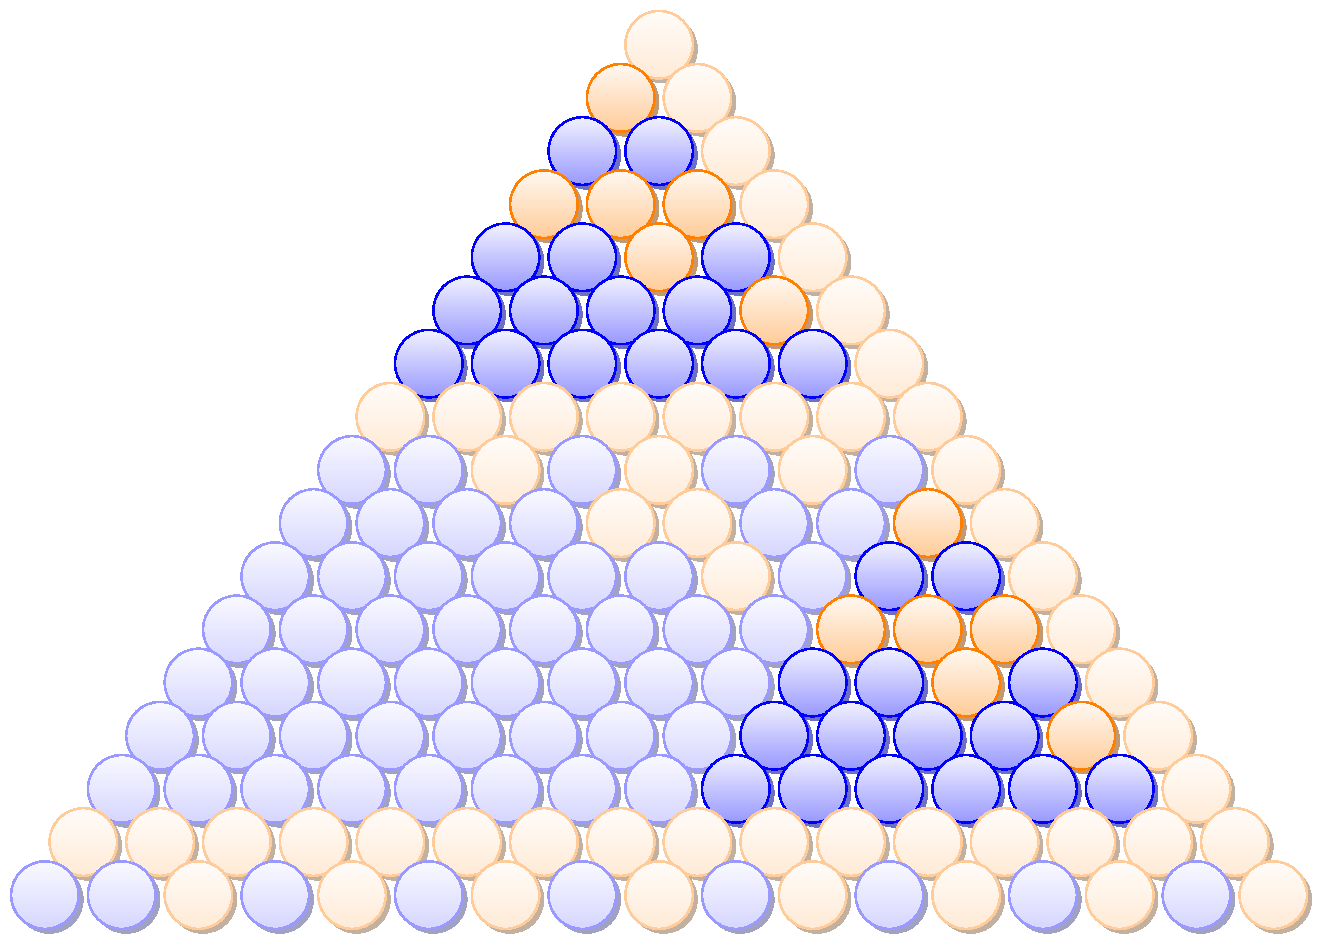
\includegraphics[width=6cm, height=6cm, keepaspectratio=true]{../RART2015/catalan-tikz/principal-cluster/principal-cluster.pdf}
    }

    % this 'particular' line is necessary to use `displaymath' environment
    % into the caption environment, togheter with the inclusion of 
    % `caption' package. See here for more explanation:
    % http://stackoverflow.com/questions/2716227/adding-an-equation-or-formula-to-a-figure-caption-in-latex
    \captionsetup{singlelinecheck=off}
    \caption[$\mathcal{C}_{\equiv_{2}}^{(4)}$ 
    contains a copy of $\mathcal{C}_{\equiv_{2}}^{(3)}$]{$\hat{d}_{s,2^{3}-1}$ for $s\in S_{2^{3}-1}$,
    $d_{s,2^{3}-1+e} \equiv_{2} d_{s-2^{3},e-1}$ with $e\in\lbrace1,\ldots,s-2^{3}\rbrace$ }

    \label{fig:catalan-principal-cluster}

\end{figure}


Before concluding the modular characterization of $\mathcal{C}$,
we would like to observe that the last two
theorems do not say anything about the \emph{value} of remainder for
a coefficient belonging to sub triangles of interest:
we have only shown that a \emph{complete} sub triangle is repeated
when coefficients are taken modulo $2$.

\subsection{A cheaper procedure to build $\mathcal{C}_{\equiv_{2}}$}

We have used \autoref{thm:mirror:segment:definition},
\autoref{thm:upside:down:zero:hole}, \autoref{thm:two:mirrored:clusters} and
\autoref{thm:principal:cluster:copy:containment} to build an efficient
procedure, written using the Python language, that builds $\mathcal{C}_{\equiv_{2}}$
inductively without resorting to the hard-way approach. The latter consists of
computing the matrix expansion of $\mathcal{C}$ by doing convolutions and
series expansion of each column, then taking each coefficient $c_{n,k}\in\mathcal{C}$ modulo 2.
On the contrary, the former uses theorems to
assemble $\mathcal{C}_{\equiv_{2}}$ block-wise: it builds a principal cluster
$\mathcal{C}_{\equiv_{2}}^{(\alpha+1)}$ consuming a principal cluster
$\mathcal{C}_{\equiv_{2}}^{(\alpha)}$, treating it as a whole block. For the sake of clarity,
let us divide $\mathcal{C}_{\equiv_{2}}^{(\alpha+1)}$ in half obtaining two strips, then the former approach acts as follows:
first, it places $\mathcal{C}_{\equiv_{2}}^{(\alpha)}$ in the top strip -- which is a triangle itself;
second, it places another copy of $\mathcal{C}_{\equiv_{2}}^{(\alpha)}$ on the very right portion in the bottom strip;
third, it mirrors last copied block respect to the mirror segment;
finally, it fills with zeros the upside-down triangle on the very left portion in the bottom strip.
Such procedure is much faster and easier to code that the one that implements definitions explicitly.
